\documentclass[aspectratio=169,11pt]{beamer}
\usepackage[T1]{fontenc}
\usepackage{booktabs}
\usepackage{amsmath}
\setbeamertemplate{navigation symbols}{}
\setbeamertemplate{footline}[frame number]
\setbeamerfont{caption}{size=\footnotesize}

\title{Super-Convergence: Very Fast Training of Neural Networks Using Large Learning Rates}
\subtitle{Leslie N.\ Smith, Nicholay Topin, arXiv:1708.07120}
\institute{HW2, Efficient Models course, ITMO 2026}
\date{}

\begin{document}

\begin{frame}
  \titlepage
\end{frame}

\begin{frame}{The claim}
  \begin{columns}[T]
    \column{0.42\textwidth}
    \begin{itemize}
      \item ResNet-56 on CIFAR-10, batch 1000
      \item Typical training: 80,000 iterations, 91.2\,\%
      \item One cycle of a large learning rate: 10,000 iterations, 92.4\,\%
      \item The authors call this \alert{super-convergence}: the same or better accuracy with an order of magnitude fewer iterations
    \end{itemize}
    \column{0.58\textwidth}
    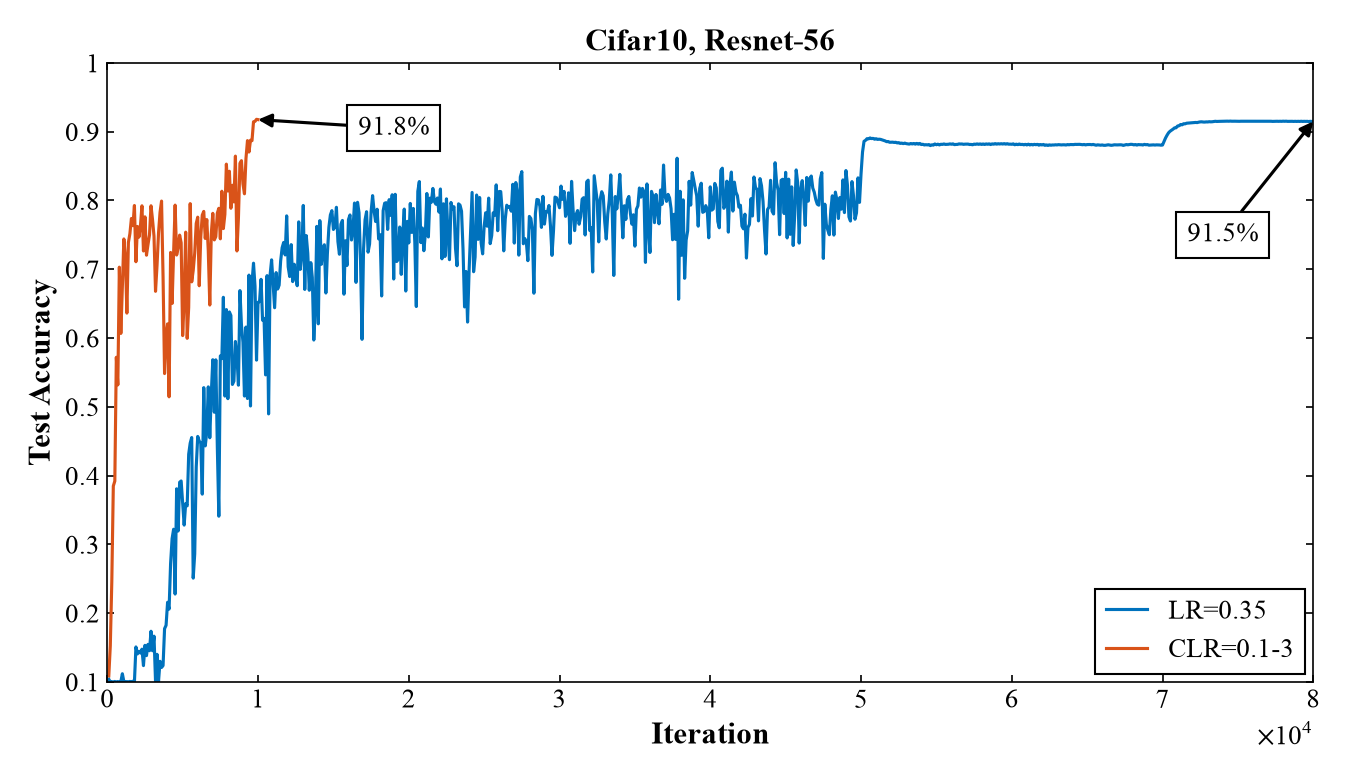
\includegraphics[width=\textwidth]{results/figures/fig1a.png}
    \centering{\footnotesize Our reproduction of Fig.\ 1a}
  \end{columns}
\end{frame}

\begin{frame}{Two learning rate schedules}
  \textbf{PC-LR}, piecewise constant, the ``typical'' baseline: LR 0.35, divided by 10 at iterations 50k and 70k.

  \medskip
  \textbf{CLR}, cyclical learning rate: LR goes linearly from \texttt{base\_lr} to \texttt{max\_lr} over \texttt{stepsize} iterations and back
  \[
    \text{lr}(t) = \text{base} + (\text{max} - \text{base}) \cdot \max\bigl(0,\ 1 - |t / s - 2c - 1|\bigr),
    \quad c = \lfloor t / 2s \rfloor, \quad s = \text{stepsize}
  \]

  \begin{itemize}
    \item Super-convergence uses one cycle, 0.1 $\to$ 3 $\to$ 0.1, stepsize 5,000
    \item LR 3 is about 30 times larger than usual for this network
    \item The paper's \alert{1cycle} policy: one cycle shorter than the run, then LR decays far below \texttt{base\_lr}
  \end{itemize}
\end{frame}

\begin{frame}{LR range test: how large can the LR be?}
  \begin{columns}[T]
    \column{0.5\textwidth}
    \begin{itemize}
      \item One short run, LR grows linearly from 0
      \item Usually test accuracy peaks and falls: the peak gives \texttt{max\_lr}
      \item ResNet-56 on CIFAR-10 has no drop up to LR 3: accuracy stays at 0.7--0.8
      \item The paper reads this as a sign that super-convergence is possible
    \end{itemize}
    \column{0.45\textwidth}
    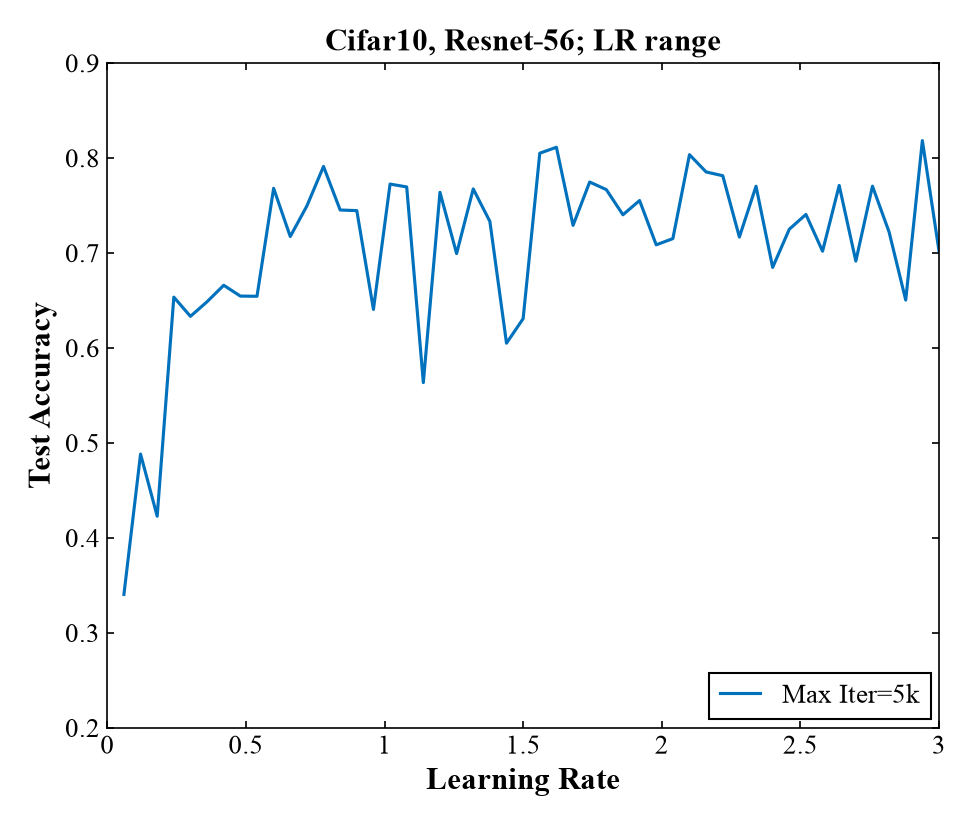
\includegraphics[width=\textwidth]{results/figures/fig2b.png}
    \centering{\footnotesize Our reproduction of Fig.\ 2b}
  \end{columns}
\end{frame}

\begin{frame}{Why it works: large learning rates regularize}
  \begin{itemize}
    \item With a large LR, SGD can't settle in sharp minima and ends in flat, wide ones, which generalize better
    \item A large LR is regularization, so other regularization has to go down: less weight decay, less dropout, larger batches
    \item The paper's rule: \alert{the amount of regularization must be balanced for each dataset and architecture}
    \item Running BN statistics have to keep up with fast-changing weights: BN moving average fraction 0.95 for CLR instead of 0.999
    \item The gain over PC-LR grows when labeled data is scarce: 80.6 vs 71.4\,\% on 10,000 training images (Table 1)
  \end{itemize}
\end{frame}

\begin{frame}{Estimating the optimal learning rate (Section 4)}
  Hessian-free view: the curvature that matters is along the SGD step. A finite difference of two gradients gives (AdaSecant)
  \[
    \epsilon^* \approx \frac{\theta_{i+1} - \theta_i}{\nabla f(\theta_{i+1}) - \nabla f(\theta_i)}
    \quad\Rightarrow\quad
    \epsilon^* = \epsilon\, \frac{\theta_{i+1} - \theta_i}{2\theta_{i+1} - \theta_i - \theta_{i+2}}
  \]
  \begin{itemize}
    \item Only weights of three consecutive iterations are needed
    \item One global estimate: sum absolute values of numerator and denominator over all weights
    \item For ResNet-56 the estimate is 2--6 in the first 300 iterations and remains high with CLR: small curvature, flat minimum
    \item The paper uses it as an illustration, not as a training method
  \end{itemize}
\end{frame}

\begin{frame}{Results in the paper}
  \begin{columns}[T]
    \column{0.5\textwidth}
    \small
    \begin{tabular}{rlr}
      \toprule
      Samples & Policy & Accuracy, \% \\
      \midrule
      50,000 & PC-LR 0.35, 80k it. & 91.2 \\
      50,000 & CLR 0.1--3, 10k it. & 92.4 \\
      40,000 & PC-LR / CLR & 89.1 / 91.1 \\
      30,000 & PC-LR / CLR & 85.7 / 89.6 \\
      20,000 & PC-LR / CLR & 82.7 / 87.9 \\
      10,000 & PC-LR / CLR & 71.4 / 80.6 \\
      \bottomrule
    \end{tabular}

    \footnotesize Fig.\ 1a and Table 1, ResNet-56, CIFAR-10
    \column{0.47\textwidth}
    Also shown in the paper:
    \begin{itemize}
      \item CIFAR-100, MNIST, ImageNet
      \item Wide ResNet, DenseNet, ResNet-50, Inception-ResNet-v2, ResNet-20/110
      \item Larger batches give a small improvement
      \item Adaptive optimizers (Nesterov, Adam, AdaDelta, AdaGrad) don't reach it
    \end{itemize}
  \end{columns}
\end{frame}

\begin{frame}{Reproduction setup}
  Following the authors' Caffe files and logs from the official repo:
  \begin{itemize}
    \item ResNet-56 from \texttt{Resnet56Cifar.prototxt}, FP32, PyTorch + Lightning
    \item Batch 1000 = 8 GPUs $\times$ 125: BN normalizes every 125 images separately
    \item Caffe SGD and LR policies, weight decay $10^{-4}$, no shuffling, random flips
    \item Kaggle, 2 $\times$ T4, one run per configuration
  \end{itemize}
\end{frame}

\begin{frame}{Results}
  \begin{columns}[T]
    \column{0.42\textwidth}
    \small
    \begin{tabular}{lrrr}
      \toprule
      Accuracy, \% & Paper & Log & Ours \\
      \midrule
      CLR, 10k it. & 92.4 & 92.4 & 91.8 \\
      PC-LR, 80k it. & 91.2 & 90.3 & 91.5 \\
      \bottomrule
    \end{tabular}
    \column{0.55\textwidth}
    \small
    \begin{itemize}
      \item 0.92 h vs 7.40 h on 2 $\times$ T4
      \item Our curves (blue) follow the authors' logs (gray), their PC-LR log is 0.9 below their paper
    \end{itemize}
  \end{columns}
  \medskip
  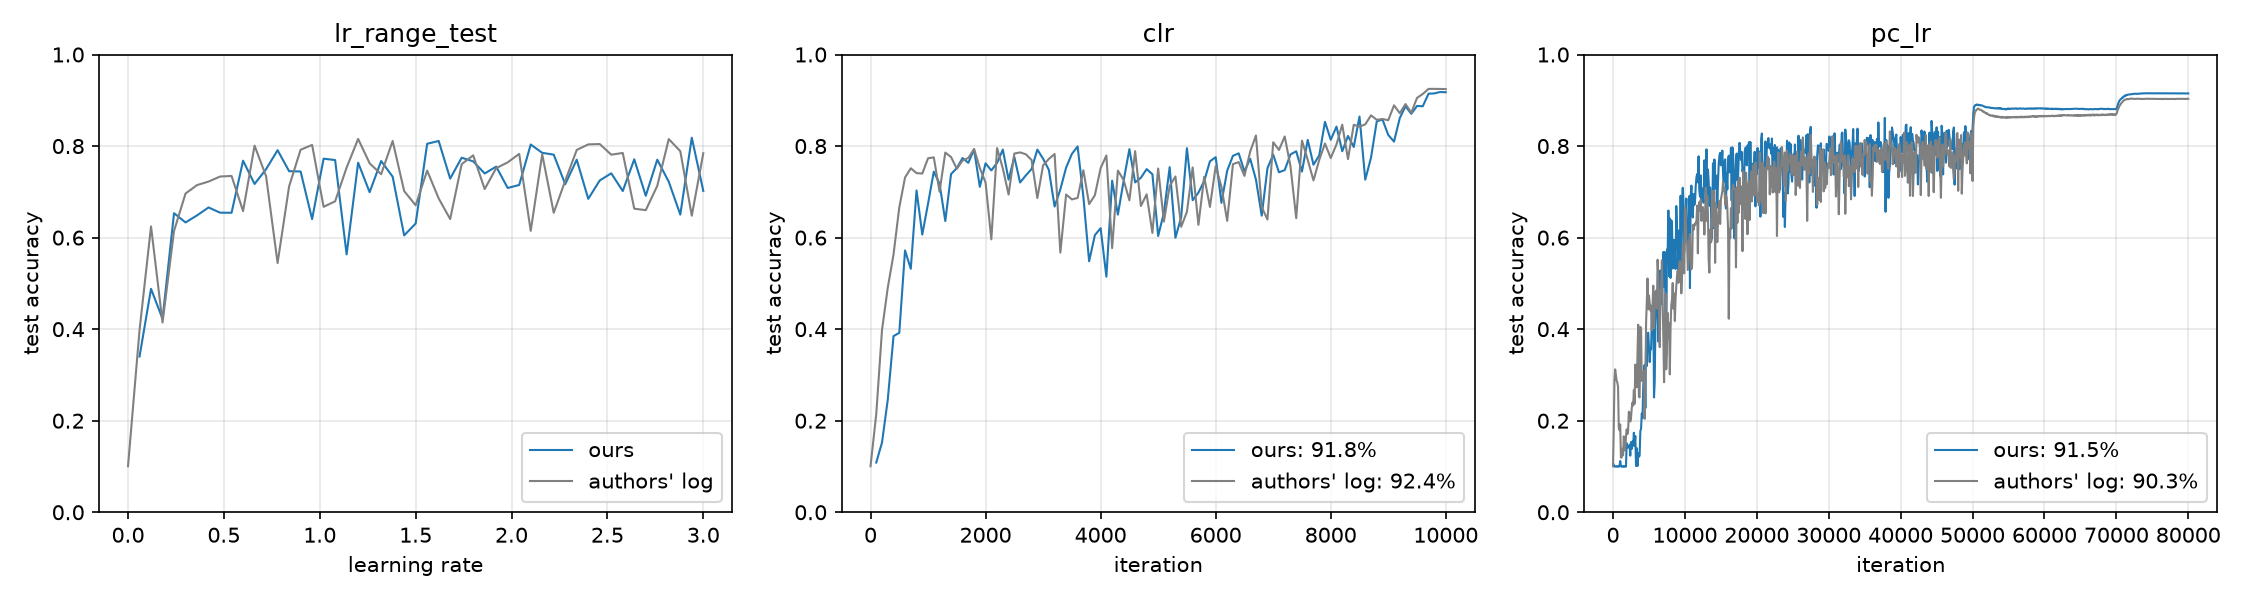
\includegraphics[width=\textwidth]{results/figures/authors_logs.png}
\end{frame}

\begin{frame}{Conclusions}
  \begin{itemize}
    \item Reproduced: one LR cycle up to 3 matches 80,000 iterations of typical training in 10,000
    \item Reproduced: the LR range test stays flat up to LR 3
    \item Not reproduced for lack of GPU time: Table 1, other stepsizes, the LR estimate, other datasets
    \item \url{https://github.com/PE51K/itmo-ai-talent-hub-efficient-models-course/tree/main/hw2}
  \end{itemize}
\end{frame}

\end{document}
